\subsubsection{Encryption - Communication} \label{section:counter-replace-encryption-content-communication}
The third approach is to use encryption on the server response as seen in figure~\ref{fig:encryptionComm}.
This additional security feature is applied in combination with a content server as described in subsection~\ref{section:counter-replace-server}.
\newline
When the user does the login on the server, additional unique device specific parameters have be passed as well, e.g. the \textit{ANDROID\_ID}.
On the first login, the server generates a cryptographic key which is used for communication with the user on this specific device.
The corresponding key can either be generated on the device or be shared by the server.
This mechanism allows only authorized users on a specific device to decrypt the communication.
\newline
\begin{figure}[h]
    \centering
    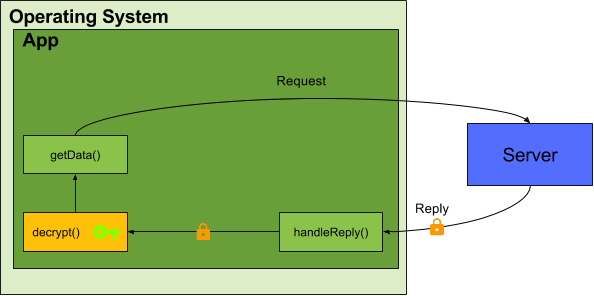
\includegraphics[width=0.8\textwidth]{data/encryptionComm.png}
    \caption{Encrypted communication with a server}
    \label{fig:encryptionComm}
\end{figure}
